\documentclass[10pt,twocolumn,letterpaper]{article}
\usepackage[margin=2.5cm]{geometry}
\usepackage{times,epsfig,graphicx,amsmath,amssymb,cite}
\usepackage[breaklinks=true,colorlinks=true,bookmarks=false]{hyperref}
\date{}

%%%%%%%%%%%%%%%%

\title{Improved Metric Learning Method Implemented in Classification Task}

\author{%
Xiaochen Zhou, Jiahao Li, Xiwen Li\\
{\tt zhouxiaochen@wustl.edu, xx@wustl.edu, xx@wustl.edu}
}


\begin{document}
\maketitle

\begin{center}\textbf{Abstract}\\~\\\parbox{0.475\textwidth}{\em
    % Abstract goes here

As a powerful method for recognition and re-identification task, metric learning greatly improve the accuracy and performance of tasks which require distance optimization between different features. Taking this property into consideration, we come out with the method to optimize the classification method with triplet loss method and improve this method to better suit the requirement of classification task. We will implement the method with convolutional neural network and make the comparison of the performance of classification between original CNN, CNN with triplet loss and CNN with our improved triplet loss.
}\end{center}

\section{Introduction}

Metric learning, highly related to similarity learning, is an area of supervised machine learning in artificial intelligence. As a powerful method to learn from examples a similarity function that measures how similar or related two objects are, metirc learning is widely use in tasks like face recognition and re-identification tasks, where the difference between special sections are much more important than the distance of the global features. Compared with classification tasks, datasets for these tasks share high similarity and the global feature supervised by softmax-entropy loss is not strong enough to clarify the difference between two faces. Metric learning method, like triplet loss which is used in this paper, is invented for further optimization. By enlarging the distance between classes, called intra-class distance and lowering the distance in the same classes, called inter-class distance, metric learning make it possible for the machine learning model to tell the difference between two similar objects.

Considering the property of metric learning, some supervising signal like triplet loss can be exerted in model training as the auxiliary loss. This method will improve the performance of classification for neural network, especially for some hardcore classification task, like sofa and chair, sofa and bed etc., which shares relatively higher similarity. Also, the auxiliary loss can cluster the classes much tighter, to some extent avoiding overfitting for the small dataset.

In this paper, we optimize triplet loss as a new supervising signal, semi-hardcore triplet loss, to help improve the performance of classification task with the assistance of convolutional neural network (CNN). Several researchers paid attention to the improvement of softmax-entropy loss function and intra-class distance optimization. Lee et.al \cite{lee2018dropmax} takes the advantages of dropout method to lower the inter-class distance. Deli{\'e}ge et.al \cite{deliege2018hitnet} developed a new hit-and-miss layer for the better performance of softmax-entropy loss. Useful as these method, new layers implemented in neural network increases the computation complexity and makes the training process longer. Using metric learning method as auxiliary loss function, however, effectively avoid the increasing computation and improve the classification performance at the same time, making the neural network training more efficient. Then, our method will improve the capability for the loss to tighten the inter-class distance and enlarge the intra-class distance.

An overview of the following sections are as follow: In section 2 we will introduce the related work on metric learning. In section 3, algorithms for our method will be given and analyzed. Then section 4 will show the performance of classification among bared softmax-entropy loss, loss with triplet loss and loss with improved triplet loss. Last section will be the conclusion.



\section{Background \& Related Work}
Feat by Xiwen Li
P.S. It should work to search information on wiki about metric learning

\section{Algorithm}
Triplet loss is first invented in Scgriff et.al \cite{schroff2015facenet}, which is exerted in face recognition task. The embedding system of triplet loss is functioning as follows. An image is set as the input of the neural network and the feature is extracted in a $d$-dimensional Euclidean space. To improve the performance of face recognition, another two images are sent into network as a triplet pair, where the original input is called image $x_i^a$ (anchor), the image sharing the same class with anchor image $x_i^p$ (positive) and the image with different class with anchor image $x_i^n$ (negative). To enlarge the inter-class distance and lower the intra-class distance, the equation can be written as follows:
$$||x_i^a - x_i^p||_2^2 + \alpha < ||x_i^a - x_i^n||_2^2, (x_i^a, x_i^p, x_i^n) \in \Gamma$$

\begin{figure}
\centering
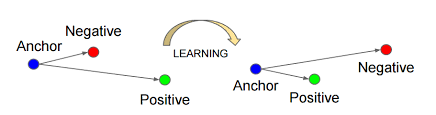
\includegraphics[width = 0.5\textwidth]{triplet.png}
\label{triplet}
\caption{Vistualization of triplet loss function}
\end{figure}

where $\alpha$ is the margin distance between positive pairs and negtive pairs and $\Gamma$ is the set of all possible triplet pairs $N$ in training period. Figure \ref{triplet} visualize the process of optimization for triplet loss. Then the loss function can be expressed as follows:
$$Loss = \sum_{i}^N [||x_i^a - x_i^p||_2^2  - ||x_i^a - x_i^n||_2^2 - \alpha]_+$$

Then to improve the performance of classification, we need to do some changes on data selection. Owing to the differences for recognition tasks are relatively small, using metric learning can making the training period unconverging. However,  considering that the difference between class in classification task is usually larger than recognition tasks, we do not need to worry too much about the negtive influence from dataset. On contrast, we need to modify the loss function, making to stronger for classification tasks.

For training period, when anchor image is set, we search the dataset to find an image  with the largest distance in the same class and to find an image with the lowest distance in different classes. The equation can be written as follows:

$$Loss = \min_{x_i^p}\max_{x_i^n} \sum_{i}^N [||x_i^a - x_i^p||_2^2  - ||x_i^a - x_i^n||_2^2 - \alpha]_+$$

\begin{figure}
\centering
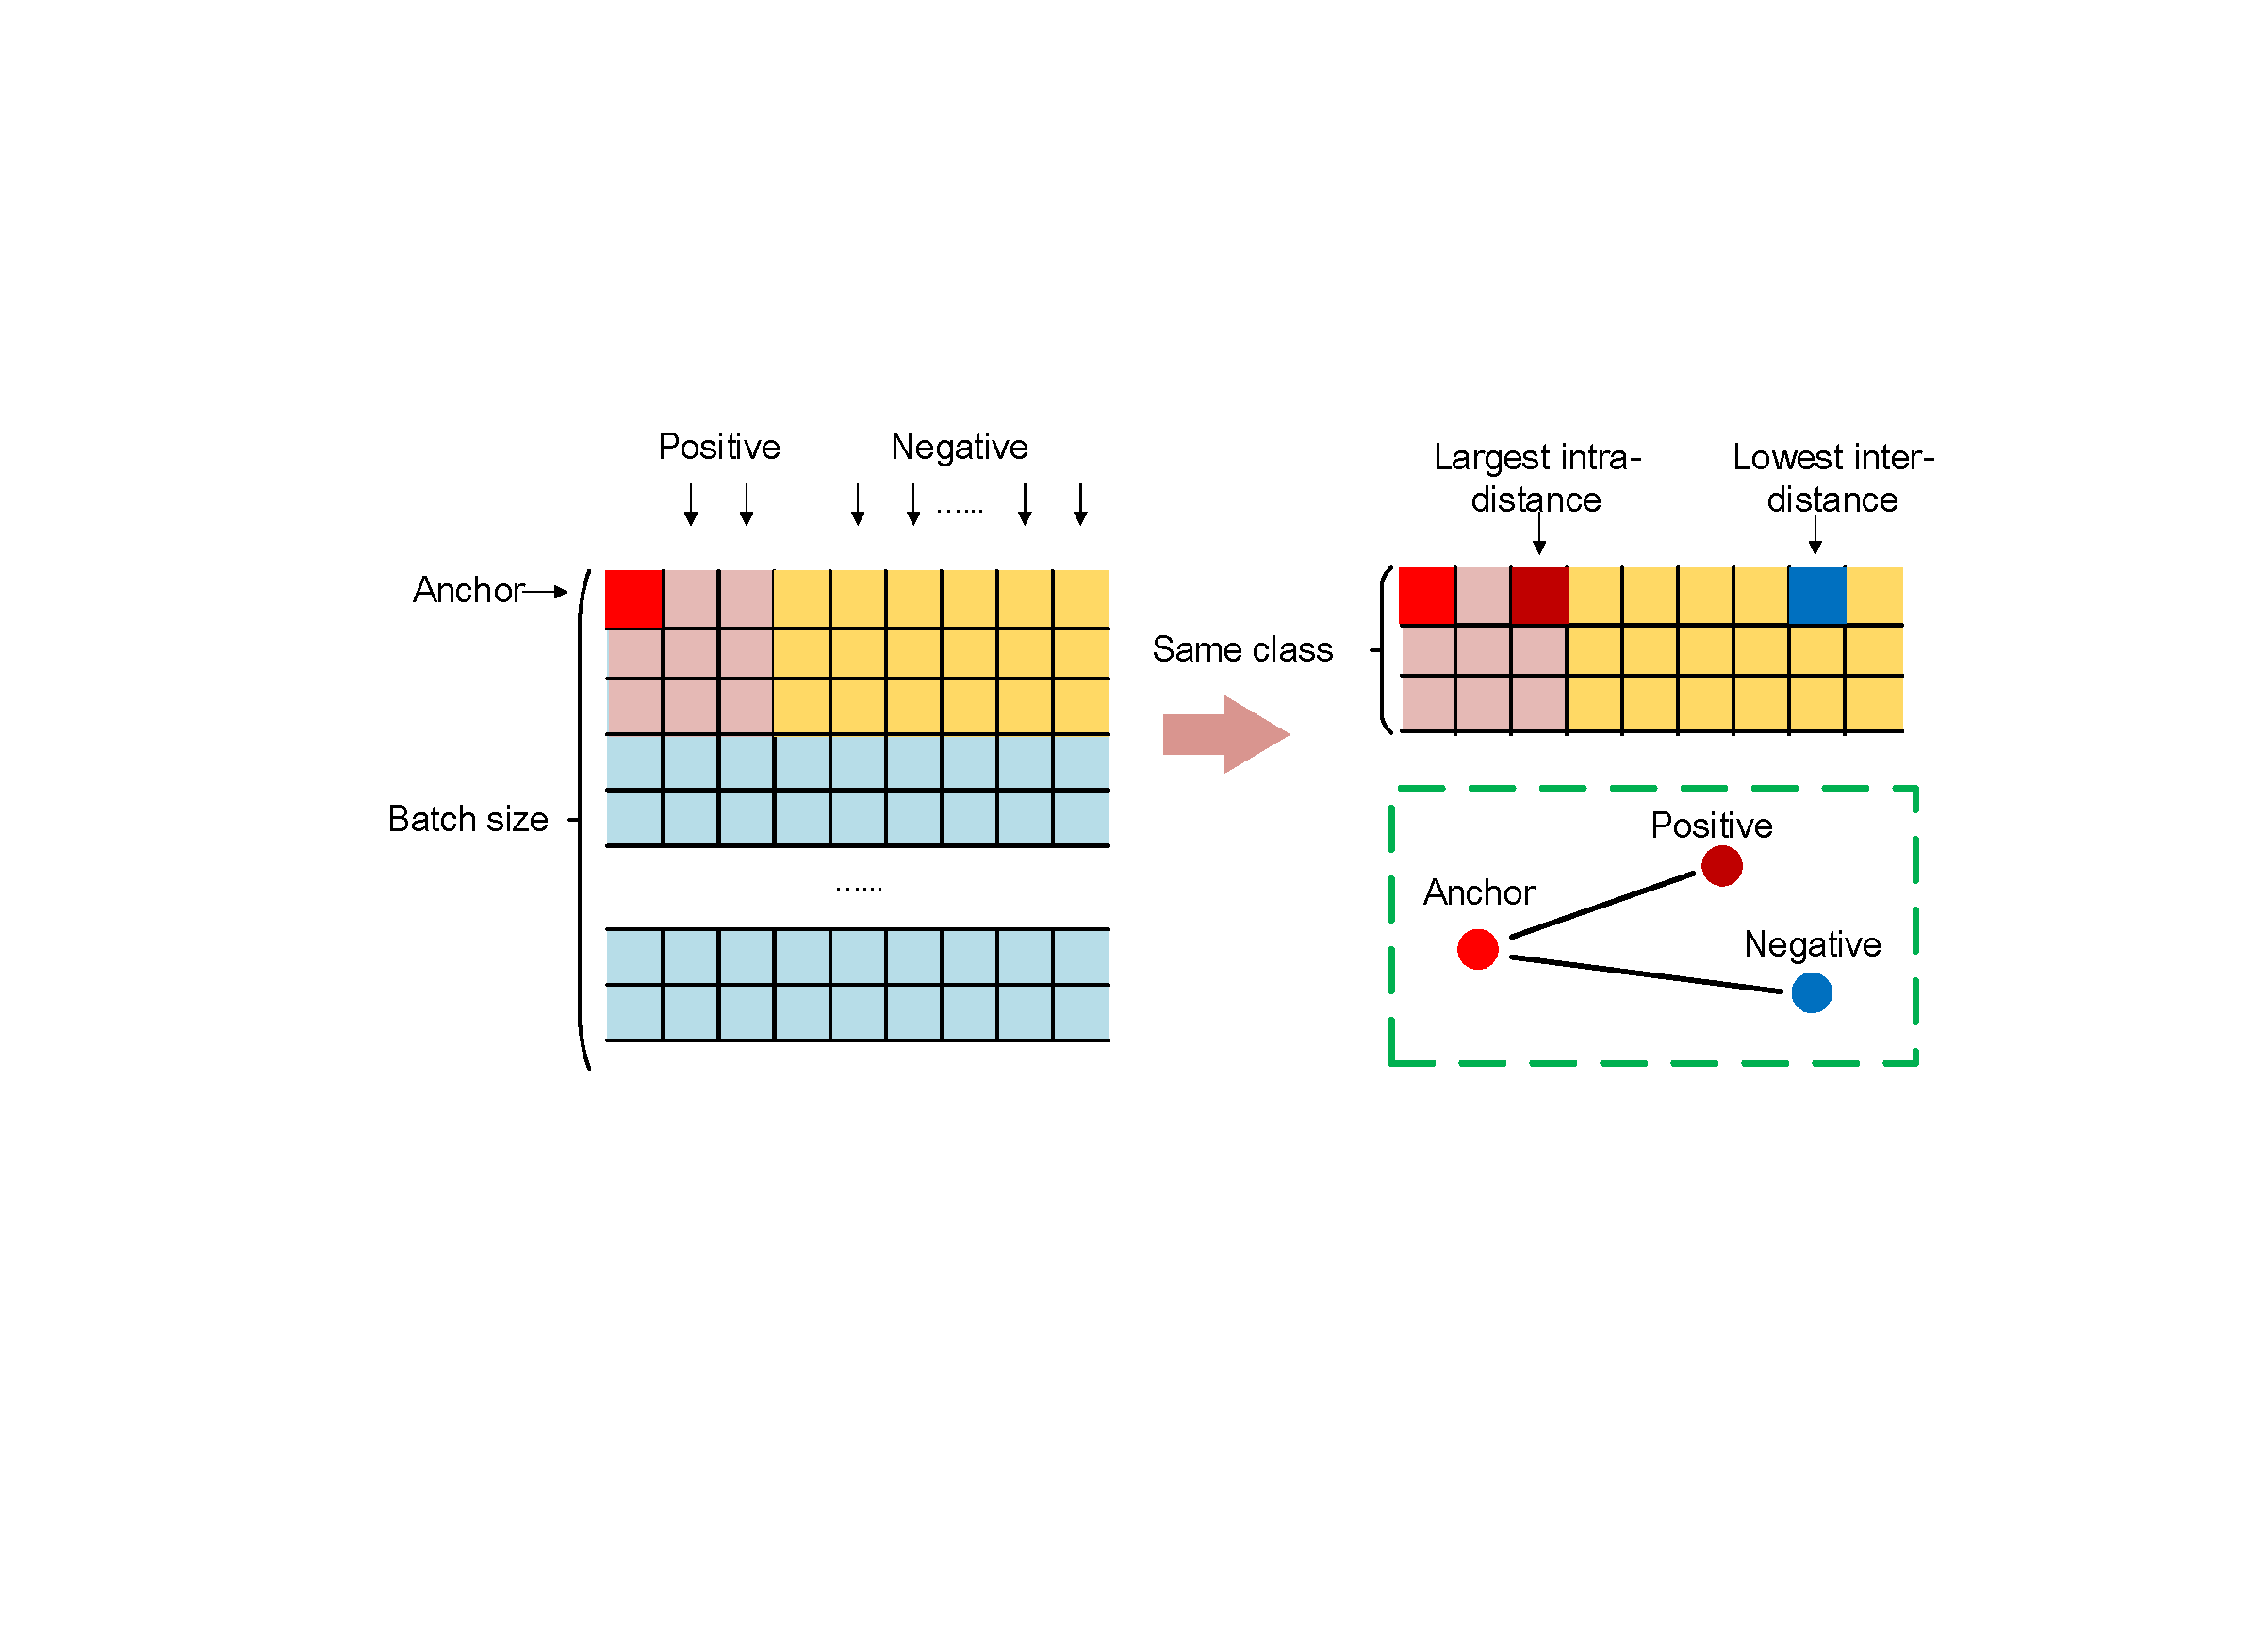
\includegraphics[width = 0.5\textwidth]{improve.pdf}
\label{improved}
\caption{Vistualization of semi-hardcore data selection for triplet loss function}
\end{figure}

This method make the loss function more hardcore than the function for recognition. However, searching for the largest distance for positive image and lowest distance for negative image is time-consuming, especially when the dataset is large. To optimize the data selection, instead of search for the whole dataset, a semi-hardcore method is implemented in this method. Considering our method is use in neural network, each time we send data into the network, we cluster the data via classes, which means, images in the same class will be gathered together. In this case, we can calculate the distance for each two images in one batch, then rank the distance to achieve the best selection in one batch. Figure \ref{improved} clarifies the process of optimization.
\section{Experimental Results}

\subsection{Dataset}
In the experiment, we implement the neural network in Caltech 101 dataset \cite{griffin2007caltech}. The number of classes is 101, about 40 to 800 images per category. Most categories have about 50 images. Collection was finished in September 2003 by Fei-Fei Li, Marco Andreetto, and Marc 'Aurelio Ranzato. The size of each image is roughly 300 x 200 pixels. For training period, 80\% of images in one class are selected as training set and 20\% of images are picked as testing set. For the baseline, we select Alexnet invented by Alex et.al \cite{NIPS2012_4824} for classification task. We extract features from the last dropout layer and send it to both fully-connection layer for softmax-entropy loss, triplet loss and semi-hardcore triplet loss as supervising signal.

\subsection{Data organization \& Experiment Environment}

Feat Xiwen Li for data organization and Experiment Environment.

(P.S. Here the experiment environment should be noticed by Jiahao)

(P.P.S Check out the data partition in section Dataset. I forget the percentage of partition for training and testing. Thanks!)

\subsection{Comparison}

Feat Jiahao Li for experiment comparison

(P.S. A table for comparison is good for visuailization. The result of improvement can be find in section Algorithm. It's ok to copy these part for comparison. Thanks!)

\section{Conclusion}
We exert a classic metric learning method, triplet loss, into classification task and do some optimzations specially for classification. Owing to the property of classification and neural network training, semi-hardcore model for data selection is used for this task. 

\section*{Acknowledgments}
Describe what sources you had help from, and so on. But try to put as much as possible as direct references in the body of the paper (like to say, ``adapting the code provided by the authors of~\cite{blah}).

{\small
\bibliographystyle{ieee}
\bibliography{refs} % Create file refs.bib, and run bibtex.
}

\end{document}
